\chapter{Teorema di Savitch} \label{ch:capitolo18}
\subsection{Teorema di Savitch}
Collega le minime risorse di memoria necessarie per risolvere deterministicamente o non deterministicamente un problema.\\\\
\textbf{Teorema}\\
Sia S un problema che si accetta non deterministicamente in spazio s dove $s(n) >= \log_2$ n è una funzione a sua volta computabile in spazio $0(s(n))$. Allora S è accettato deterministicamente in spazio $0(s2(n)).$\\\\
\textbf{Corollario}\\
\begin{center}
    PSPACE = NPSPACE
\end{center}
\begin{center}
    $L \subseteq NL \subseteq P \subseteq NP \subseteq PSPACE = NPSPACE$
\end{center}
\subsection{Gap}
\textbf{Proposizione}\\
Il problema GAP può essere accettato deterministicamente in spazio $0(log^2 n)$.\\\\
\textbf{Dimostrazione}\\
Sia G = (V , E) un grafo diretto finito.\\
Consideriamo la funzione Acc: $V x V x N \mapsto B$ definita da
\begin{figure}[htp]
    \centering
    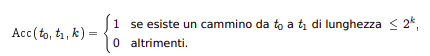
\includegraphics[scale=0.9]{tesi_stile/img/foto1cap18.png}
\end{figure}
\\Si verifica facilmente che:
\begin{figure}[htp]
    \centering
    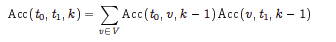
\includegraphics[scale=0.9]{tesi_stile/img/foto2cap18.png}
\end{figure}
\begin{figure}[htp]
    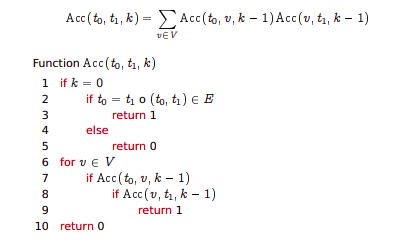
\includegraphics[scale=0.8]{tesi_stile/img/foto3cap18.png}
\end{figure}
\newpage
\subsection{Analisi}
\begin{figure}[htp]
    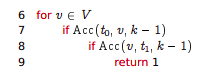
\includegraphics[scale=0.8]{tesi_stile/img/foto4cap18.png}
\end{figure}
Sia $s_k$ lo spazio per l’esecuzione dell’algoritmo.\\
La variabile v richiede spazio $\log_2 n$.\\
L’istruzione 2 richiede spazio $s_k-1$.\\
L’istruzione 3 può essere eseguita nello spazio già usato per l’istruzione 2.\\
Se ne deduce $sk = s_k-1 + \log_2n$ e, risolvendo la ricorrenza.\\
\begin{center}
    $s_k = k log_2 n$
\end{center}
\subsection{Conclusione}
Detto n il numero di vertici di G e k = $|log_2 n|$, si ha $(G,t_0,t_1)$ $\in$ GAP se e solo se $Acc(t_0,t_1, k) = 1$. Quindi il problema si risolve in spazio
\begin{itemize}
    \item $klog_2 n <= (log_2 n)^2$
\end{itemize}
\subsection{Il caso NL}
\textbf{Proposizione}\\
Sia $S \in NL$. Allora S è accettato deterministicamente in spazio $0((log_2n)^2)$.\\\\
\textbf{Dimostrazione}\\
Adattando le tecniche sviluppate nelle lezioni precedenti, si ha che se $S <=_{\log} T$ e T si calcola in spazio $O(log^2 n)$, allora anche S si calcola in spazio $O(log^2 n)$. Poichè GAP è NL-completo, si ha $S <=_{log}$ GAP e l’asserto segue dal lemma precedente.
\subsection{Il caso generale}
Sia M una macchina di Turing che accetta S in spazio s(n).\\
Osserviamo che si ha w $\in$ S se e solo se c’è un cammino nel grafo G(M, w) dalla configurazione iniziale alla configurazione di arresto.
\\Adattando l’algoritmo usato per GAP, si può verificare questa condizione in
spazio $O(s^2(n))$.
\subsection{Il complemento di GAP}
\textbf{Lemma}
\begin{center}
    GAP $\in$ coNL
\end{center}
\textbf{Dimostrazione}\\
Dobbiamo trovare una procedura non deterministica che accetta in spazio logaritmico il complemento di GAP.\\
Sia G = (V , E) un grafo diretto e $t_0 \in V$ un vertice. Per ogni intero j $>=$ 0,
diremo che un vertice v $\in$ V è j -accessibile se esiste un cammino di lunghezza j da $t_0$ a v.
\subsection{Vertici j-accessibili}
Supponiamo di conoscere il numero r dei vertici j -accessibili.
\\Allora possiamo realizzare una procedura non deterministica, che ci dice se un dato vertice v è $(j+1)-$accessibile o meno.
\\Invero, possiamo procedere nel modo seguente:
\begin{itemize}
    \item Per ogni vertice u $\in$ V , generiamo non deterministicamente un cammino di lunghezza j che parte da $t_0$ 
    \item Se il numero dei vertici u per cui il cammino generato termina proprio in u è uguale a r , allora possiamo concludere che gli u per cui questo avviene sono esattamente i vertici j -accessibili; in tal caso, il vertice v è $(j+1)-$accessibile se e solo se v è adiacente a uno di tali vertici
    \item Se invece il numero delle volte in cui il cammino generato termina in u è minore di r , allora non possiamo concludere nulla.
\end{itemize}
\newpage
\subsection{Procedura Accesso}
\textbf{Input:} Un grafo diretto $G = (V , E), t_0$, $v \in V$ , $j >= 0$, r = numero dei vertici j-accessibili.
\\Output: \textbf{VERO} se v è $(j+1)-$accessibile, \textbf{FALSO} altrimenti (nelle esecuzioni che terminano)
\begin{figure}[htp]
    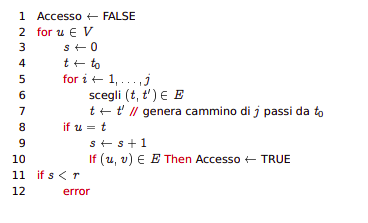
\includegraphics[scale=0.7]{tesi_stile/img/foto5cap18.png}
\end{figure}
\subsection{Calcolo di r}
Ora siamo in grado di calcolare il numero dei vertici j -accessibili per j = $1, 2,..., n-1$. Invero, una volta calcolato il numero r dei vertici j-accessibili, applicando la procedura Accesso a tutti i vertici v $\in$ V , potremo conoscere il numero dei vertici $(j+1)$-accessibili.
\\\textbf{Procedura ContaAccessibili}\\
\textbf{Input:} Un grafo diretto G = (V , E), $t_0$ $\in$ V.
\\\textbf{Output:} Genera il numero r dei vertici (j+1)-accessibili per ogni j.
\begin{figure}[htp]
    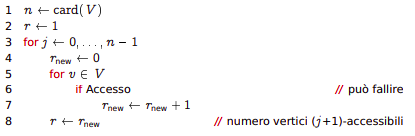
\includegraphics[scale=0.7]{tesi_stile/img/calcolo-di-r.png}
\end{figure}
\newpage
\subsection{Accettare il complemento di GAP}
Una semplice modifica del procedimento permette anche di determinare se
un vertice è inaccessibile.
\\Otteniamo così la seguente procedura che può terminare solo se $t_1$ è
inaccessibile da $t_0$.
\begin{figure}[htp]
    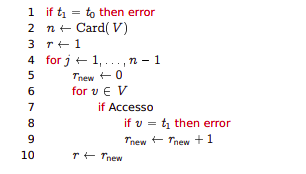
\includegraphics[scale=0.7]{tesi_stile/img/accertare-gap.png}
\end{figure}
\subsection{NL = coNL}
\textbf{Teorema}
\begin{center}
    NL = coNL
\end{center}
\textbf{Dimostrazione}
\begin{figure}[htp]
    \centering
    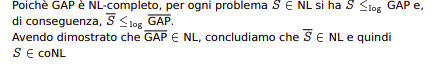
\includegraphics[scale=0.8]{tesi_stile/img/foto9cap18.png}
\end{figure}
\newpage
\section{NL = coNL Approfondito}
Vogliamo mostrare che le classi di complessità spaziale NL e coNL coincidono. Il primo passo consiste nel mostrare che il problema NL-completo GAP sta nella classe coNL.\\\\
\textbf{Lemma 1}
\begin{center}
    $GAP \in coNL$
\end{center}
\textbf{Dimostrazione}\\
Per dimostrare l’asserto dobbiamo trovare una procedura non deterministica che accetta in spazio logaritmico il complemento di GAP, ossia l’insieme delle triple $(G, t_0, t_1)$, ove G è un grafo diretto e $t_0$ e $t_1$ sono due vertici di G con $t_1$ inaccessibile da $t_0$.
\\Sia dunque G = (V, E) un grafo diretto e $t_0 \in V$ un vertice. Per ogni intero $j >= 0$, diremo che un vertice $v \in V$ è j-accessibile se esiste un cammino di lunghezza j da $t_0$ a v. Supponiamo di conoscere il numero r dei vertici j-accessibili.
\\ Allora possiamo realizzare una procedura non deterministica, che ci dice se un dato vertice v è (j + 1)-accessibile o meno. Invero, possiamo procedere nel modo seguente:
\begin{itemize}
    \item Per ogni vertice u $\in$ V, generiamo non deterministicamente un cammino di lunghezza j che parte da $t_0$ 
    \item Se il numero dei vertici u per cui il cammino generato termina proprio in u è uguale a r, allora possiamo concludere che gli u per cui questo avviene sono esattamente i vertici j-accessibili; in tal caso, il vertice v è (j + 1)-accessibile se e solo se v è adiacente a uno di tali vertici
    \item Se invece il numero delle volte in cui il cammino generato termina in u è minore di r, allora non possiamo concludere nulla.
\end{itemize}
Abbiamo così a disposizione la seguente procedura non deterministica che per ogni vertice v termina almeno una volta determinando correttamente se v è (j + 1)-accessibile o non lo è.
\begin{figure}[htp]
    \centering
    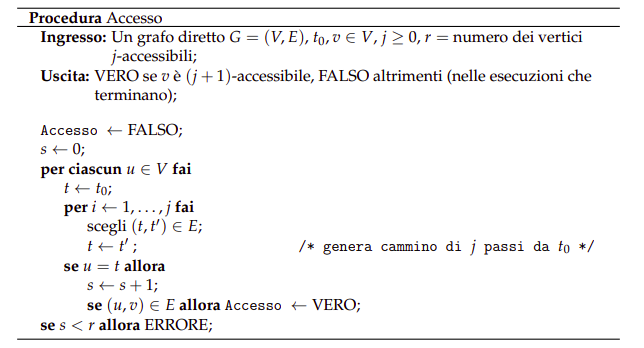
\includegraphics[scale=0.6]{tesi_stile/img/nl1.png}
\end{figure}
\\Ora siamo in grado di calcolare il numero dei vertici j-accessibili per $j =1,2, ...,n - 1$. Invero, una volta calcolato il numero r dei vertici j-accessibili, applicando la procedura Accesso a tutti i vertici $v \in V$, potremo conoscere il numero dei vertici (j + 1)-accessibili.
\\La procedura è la seguente:
\begin{figure}[htp]
    \centering
    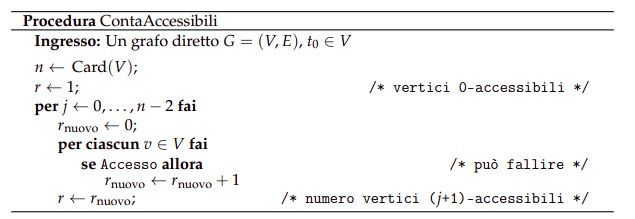
\includegraphics[scale=0.6]{tesi_stile/img/nl2.png}
\end{figure}
\\Naturalmente, in molte esecuzioni del procedimento testé descritto, qualche chiamata a Accesso determinerà un errore. Esiste però almeno una esecuzione in cui tutte
le chiamate terminano correttamente. In tal caso, il procedimento determina esattamente tutti i vertici j-accessibili per $j = 1, 2, ... , n - 1$. Tenuto conto che in un grafo con n vertici, un vertice è accessibile se e solo se è j-accessibile per qualche $j < n$, una semplice modifica del procedimento permette anche di determinare se un vertice è inaccessibile. Otteniamo così la seguente procedura che può terminare solo se $t_1$ è inaccessibile da $t_0$.
\begin{figure}[htp]
    \centering
    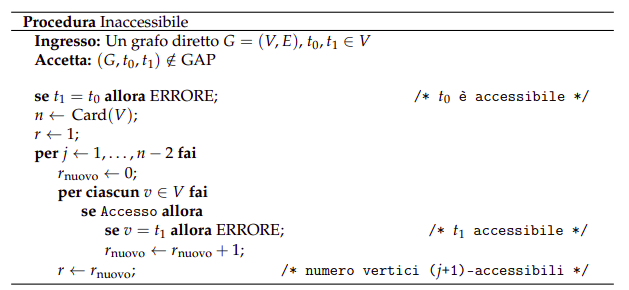
\includegraphics[scale=0.6]{tesi_stile/img/nl3.png}
\end{figure}
\\Adesso occupiamoci di studiare la complessità spaziale della procedura Inaccessibile.
\\Tale procedura fa uso delle variabili n, r, $r_{nuovo}$, v, ciascuna delle quali richiede spazio logaritmico rispetto al numero dei vertici di G, e inoltre necessita dello spazio per l’esecuzione della procedura accesso. Anche le variabili della procedura Accesso richiedono spazio logaritmico rispetto al numero dei vertici di G. Possiamo concludere quindi che $GAP \in coNL$.
\\Ora utilizzeremo il fatto che $GAP \in coNL$ per mostrare che $NL = coNL$. \\Iniziamo col seguente:\\\\
\textbf{Lemma 2}\\
Siano S e T due problemi. Se $S <=_{\log} T$ e $T \in coNL$, allora $S \in coNL$.\\\\
\textbf{Dimostrazione}\\    
Si osservi che una riduzione f di S a T è anche una riduzione del complemento $\Bar{S}$ di S al complemento $\Bar{T}$ di T. Quindi se $S <=_{\log}T$, si ha anche $\Bar{S} <=_{\log}\Bar{T}$.
\\Tenuto conto del fatto che $T \in NL$, si ha $S \in NL$ e quindi $S \in coNL$.
\\Ora siamo pronti per dimostrare il nostro risultato principale.\\\\
\textbf{Teorema 1}
\begin{center}
    NL = coNL
\end{center}
\textbf{Dimostrazione}\\
Sia S $\in$ NL. Poiché GAP è NL-completo, si ha $S <=_{\log} GAP$ e quindi, per i lemmi precedenti, S $\in$ coNL.
\\Viceversa, sia S $\in$ coNL. Allora il suo complemento S sta in NL. Per l’argomento precedente, si ha S $\in$ coNL e quindi S $\in$ NL. Se ne conclude che le classi NL e coNL coincidono.